\documentclass[12pt, letterpaper, twoside]{article}

% Paquetes básicos
\usepackage[utf8]{inputenc}
\usepackage[spanish, es-tabla]{babel}
\usepackage{graphicx}
\usepackage{amsmath}
\usepackage{amsthm}
\usepackage{comment}
\usepackage{hyperref}
\hypersetup{pdftex,colorlinks=true,allcolors=black}

% Referencias
\usepackage[backend=biber, bibstyle=authoryear, citestyle=authoryear]{biblatex}
\addbibresource{referencias.bib}

% Configuraciones de formato
% Configuración de formato para tesina BANGUAT 2016

% Márgenes
\usepackage{geometry}
\geometry{letterpaper, margin=1in, left=3cm}

% Numeración a los ambientes \paragraph y profundidad del índice
\setcounter{secnumdepth}{4}
\setcounter{tocdepth}{3}

% Formato de las secciones y subsecciones
%\usepackage{titlesec}
%\titleformat*{\section}{\large\bfseries}
%\titleformat*{\subsection}{\normalsize\bfseries}
%\titleformat{\section}{\normalfont\scshape}{\thesection}{1em}{}
%\titleformat{\section}[block]{\large\bfseries}{\thesection.}{0.5cm}{}

% Letra arial
\usepackage{helvet}
\renewcommand{\familydefault}{\sfdefault}

% Indentado
\setlength\parindent{1cm}

% Interlineado 1.5
\renewcommand{\baselinestretch}{1.5}

% Fuente para la mate
\usepackage[osf,sc]{mathpazo}
\usepackage{eulervm}

% Fuente para las gráficas y tablas
\usepackage{caption}
\captionsetup{
	labelfont=bf,
	textfont={normalsize},
	justification=centering}

% Líneas para las tablas
\usepackage{multirow}
\usepackage{booktabs}
% Para poner el largo de la tabla
\usepackage{tabularx}

% Configuración de listings
% Paquetes necesarios
\usepackage{listingsutf8}
\usepackage{color}

% Redefinición de titulos de caption
\renewcommand\lstlistingname{Código}
\renewcommand\lstlistlistingname{Índice de códigos}

% Definición de colores para R
\definecolor{frame_numbers_color}{rgb}{0.5,0.5,0.5}

\definecolor{r_comment_color}{RGB}{221, 0, 221}
\definecolor{r_string_color}{RGB}{0, 170, 0}
\definecolor{r_keyword_color}{RGB}{255, 119, 0}
\definecolor{r_identifier_color}{RGB}{0,0,0}

% Definicion de estilo para R
\lstdefinestyle{customR}{
	backgroundcolor=\color{white},   % choose the background color;
	%basicstyle=\footnotesize,        % the size of the fonts that are used for the code
	basicstyle=\small\ttfamily,
	breakatwhitespace=false,         % sets if automatic breaks should only happen at whitespace
	breaklines=true,                 % sets automatic line breaking
	captionpos=t,                    % sets the caption-position to bottom
	commentstyle=\color{r_comment_color},    % comment style
	deletekeywords={...},            % if you want to delete keywords from the given language
	escapeinside={\%*}{*)},          % if you want to add LaTeX within your code
	extendedchars=true,              % lets you use non-ASCII characters; for 8-bits encodings only, does not work with UTF-8
	frame=single,                    % adds a frame around the code
	framesep=3pt,
	identifierstyle=\color{r_identifier_color},
	keepspaces=true,                 % keeps spaces in text, useful for keeping indentation of code (possibly needs columns=flexible)
	keywordstyle=\mdseries\color{r_keyword_color},       % keyword style
	language=R,                 % the language of the code
	morekeywords={},            % if you want to add more keywords to the set
	numbers=left,                    % where to put the line-numbers; possible values are (none, left, right)
	numbersep=7pt,                   % how far the line-numbers are from the code
	numberstyle=\tiny\color{frame_numbers_color}, % the style that is used for the line-numbers
	rulecolor=\color{black},         % if not set, the frame-color may be changed on line-breaks within not-black text (e.g. comments (green here))
	showspaces=false,                % show spaces everywhere adding particular underscores; it overrides 'showstringspaces'
	showstringspaces=false,          % underline spaces within strings only
	showtabs=false,                  % show tabs within strings adding particular underscores
	stepnumber=1,                    % the step between two line-numbers. If it's 1, each line will be numbered
	stringstyle=\color{r_string_color},     % string literal style
	tabsize=4,                       % sets default tabsize to 2 spaces
	title=\lstname                   % show the filename of files included with \lstinputlisting; also try caption instead of title	
}
\lstset{style=customR, frame=none}


% Para la bibliografía
%\setlength\bibitemsep{1.5\itemsep}
\setlength\bibitemsep{\baselineskip}

% Doble enter después de párrafos
%\nonfrenchspacing

% Para evitar que deje secciones al final de la página
\begin{comment}
\usepackage{etex}
\usepackage{etoolbox}
\makeatletter
\patchcmd{\@afterheading}%
{\clubpenalty \@M}{\clubpenalties 3 \@M \@M 0}{}{}
\patchcmd{\@afterheading}%
{\clubpenalty \@clubpenalty}{\clubpenalties 2 \@clubpenalty 0}{}{}
\makeatother

% Otra posible solución con needspace:

\usepackage{titlesec}
\usepackage{needspace}
...
\titleformat{\section}
{\needspace{1in}\Large\bfseries}{\thesection}{1em}{}

\end{comment}




\begin{document}
	
	% Carátula del documento
	% Titulo del documento
\title{Modelo de pronóstico del tipo de cambio para Guatemala utilizando redes neuronales artificiales}
\author{Rodrigo Chang}
\date{julio de 2016}

\thispagestyle{empty}
\pagenumbering{gobble}
\noindent
\maketitle

	
	% Índice de contenidos, figuras y tablas
	\pagenumbering{Roman}
	\setcounter{page}{1}
	% Índice del documento

\tableofcontents
\newpage
\listoffigures
\listoftables
%\lstlistoflistings
\newpage
	
	% Cuerpo del documento
	\pagenumbering{arabic}
	\setcounter{page}{1}
	
	% Resumen e introducción
	\section*{Resumen}
\addcontentsline{toc}{section}{Resumen}
El tipo de cambio es una de las variables macroeconómicas más importantes debido a que tiene influencia en las decisiones tomadas por los participantes del mercado de divisas como lo son los inversores, importadores, exportadores, banqueros e instituciones financieras, turistas y hacedores de política. Es por esto que un pronóstico adecuado del tipo de cambio resulta una herramienta invaluable para dichos agentes económicos.\\

De acuerdo con la literatura, el pronóstico del tipo de cambio a través de modelos que utilizan fundamentos macroeconómicos está desestimado desde el trabajo seminal presentado por \textcite{meese1983empirical}, en el cual ningún modelo de pronósticos logra superar a un modelo de caminata aleatoria. Desde entonces, han sido muchas las técnicas y modelos utilizados para intentar mostrar que los fundamentos macroeconómicos pueden determinar el tipo de cambio.\\

Entre estas técnicas se han utilizado variantes no lineales, como las redes neuronales artificiales, que han tenido un reciente auge en la resolución de problemas de distintas displinas. En este trabajo se pretende responder a la interrogante ¿Es posible pronosticar el tipo de cambio utilizando una red neuronal que incorpore fundamentos macroeconómicos? En tal sentido, se tiene como objetivo determinar la efectividad de un modelo pronóstico del tipo de cambio para Guatemala utilizando redes neuronales que incorporen agregados macroeconómicos, y comparar los resultados con un modelo de caminata aleatoria y un modelo lineal con los mismos fundamentos.\\

Finalmente, derivado del trabajo de investigación se determina que para Guatemala los modelos que utilizan fundamentos macroeconómicos pronostican mejor el tipo de cambio, y que en general, el modelo de redes neuronales provee mejores medidas de pronóstico que el modelo lineal y el modelo de caminata aleatoria.
% afirmando que es posible la predicción del tipo de cambio a través de fundamentos macroeconómicos.

\newpage
\section*{Introducción}
\addcontentsline{toc}{section}{Introducción}

El tipo de cambio, que es el precio de una moneda extranjera expresado en la moneda local, afecta el comportamiento de los agentes económicos que intervienen en el mercado de divisas y tiene repercusiones en la economía en general. En la actualidad, debido al alto grado de globalización y la apertura económica de los países, el tipo de cambio juega un rol crucial en el movimiento de capital extranjero y en el comercio internacional.\\

Desde la caída del sistema Bretton Woods (que imponía un tipo de cambio fijo) a inicios de los años setenta, la predicción del tipo de cambio se ha vuelto más relevante ya que tiene importancia en aspectos prácticos, porque permite a inversores, bancos centrales e instituciones financieras decidir la asignación de activos, manejar el riesgo y formular políticas. Además, la significancia teórica del pronóstico del tipo de cambio tiene implicaciones vitales en la hipótesis de mercados eficientes, así como el desarrollo de modelos teóricos en finanzas internacionales.\\

Para modelar el comportamiento del tipo de cambio se han utilizado a lo largo del tiempo distintos modelos que emplean variables macroeconómicas para explicar la tendencia y volatilidad en el tipo de cambio. Entre estos se encuentran dos clases generales de modelos, el monetario y el de cartera de balance. Ambos utilizan supuestos como la paridad de poder adquisitivo, y la paridad de los tipos de interés para explicar los movimientos en el tipo de cambio.\\

En la literatura, los modelos estructurales (con fundamentos macroeconómicos) de pronóstico del tipo de cambio se vieron frustrados cuando \textcite{meese1983empirical} presentan un trabajo contundente sobre los el tipo de cambio, en el cual encuentran que un modelo de caminata aleatoria simple podía pronosticar mejor el tipo de cambio que una serie de modelos estructurales. Desde entonces los investigadores han desarrollado todo tipo de modelos teóricos y empleado técnicas de pronóstico poderosas para tener un mejor entendimiento acerca del movimiento de los tipos de cambio y para intentar vencer al modelo de caminata aleatoria. Además, el modelo monetario plantea una relación lineal en los determinantes del tipo de cambio, e ignora componentes no lineales que pueden darse en las observaciones reales, y debido a esto, se han utilizado métodos que capturen las componentes no lineales observados en los datos.\\

Entre los distintos trabajos de pronóstico del tipo de cambio, \textcite{sunythesis} utiliza un modelo monetario con variables como el ingreso real relativo entre dos países, la oferta monetaria relativa, el diferencial de tasas de interés y el diferencial de inflación para entrenar una red neuronal artificial y pronosticar exitosamente el tipo de cambio a través de los fundamentos macroeconómicos.\\

Una red neuronal es un método general de captura de las componentes no lineales entre variables, inspirado en la forma en que está compuesto el sistema nervioso humano, empleando neuronas interconectadas para aprender el patrón de comportamiento entre las variables de entrada y proveer un estímulo de salida, que puede ser utilizado en problemas de clasificación y regresión de variables.\\

Debido a los problemas de pronóstico que se han presentado en los trabajos de tipo de cambio a lo largo de la historia, y dado el reciente auge de la utilización de redes neuronales en la resolución de problemas en distintas disciplinas, se justifica la utilización de un modelo de regresión empleando redes neuronales y variables que de acuerdo a los modelos teóricos determinen el tipo de cambio para evaluar la eficacia de un pronóstico empleando esta técnica.\\

En el presente trabajo se emplea una metodología cercana a la presentada por \textcite{sunythesis}, en la cual se replica un modelo de caminata aleatoria utilizando la serie del tipo de cambio del quetzal contra el dólar estadounidense para pronosticar el tipo de cambio y evaluar este pronóstico contra uno dado por modelos estructurales, específicamente del modelo monetario, empleando el modelo lineal convencional y empleando la técnica de redes neuronales artificiales.\\

En el primer capítulo se describen los fundamentos teóricos del tipo de cambio y los modelos teóricos que se han empleado en la explicación de movimientos en el tipo de cambio, así como los supuestos de los que parten dichos modelos.\\

En el segundo capítulo se describe con mayor precisión la metodología empleada para el ajuste de los modelos monetarios, así como una breve descripción de los aspectos técnicos relacionados con el entrenamiento de la red neuronal, y las medidas de evaluación de pronósticos que se utilizarán para comparar dichos los modelos.\\

En el tercer capítulo se describen los pronósticos obtenidos utlizando los distintos modelos y se interpretan los resultados de acuerdo con la teoría económica.\\

Finalmente en el cuarto capítulo se hacen observaciones sobre los hallazgos clave obtenidos en la investigación.
	
	% Marco teórico
	% [y] Mencionar de que el tipo de cambio más importante para Guatemala es el dólar.
	% [y] Revisar comentarios de Rosa.
		\section{Marco teórico}
	
	% definición
	% importancia del estudio del tipo de cambio en otras variables
	% modelos o teorías disponibles que lo han estudiado
	% evolución histórica mundial del tipo de cambio y luego local
	
	\subsection{El tipo de cambio} 
	El tipo de cambio se puede definir como el precio de la moneda de un país en función de la moneda de otro. Debido a su fuerte impacto sobre la cuenta corriente y otras variables macroeconómicas, el tipo de cambio es uno de los precios más importantes de una economía abierta. El papel del tipo de cambio en el comercio internacional es fundamental, porque permite comparar los precios de bienes y servicios producidos en diferentes países. \parencite{intecon}. La anterior definición implica que un incremento en el tipo de cambio representa una depreciación de la moneda local, y un decremento en el tipo de cambio representa una apreciación de la moneda local. \parencite{exchecon}\\
	
	% El tipo de cambio se expresa como el número de unidades de moneda nacional que hay que entregar para obtener una unidad de moneda extranjera. 
	
	% Mercado de divisas
	Las transacciones entre monedas de diferentes países se llevan a cabo en el mercado de divisas, y son las que determinan el precio o tipo de cambio de una moneda respecto a otra. Una divisa es toda moneda extranjera usada en un país o región diferente del país donde se expide. \parencite{mochon}\\
	
	En el mercado de divisas se distinguen dos segmentos en función del tiempo entre el inicio y el cierre de las transacciones, que configuran dos grupos específicos de operaciones y dos precios o tipos de cambio: el tipo de cambio \textit{spot} y el tipo de cambio a plazo (\textit{forward}). En el mercado \textit{spot} se realizan operaciones de compra y venta de divisas, y la entrega se realiza dos días hábiles posteriores al de contratación, mientras que en el mercado a plazo la liquidación se realiza en el futuro, a partir del tercer día hábil posterior al de la contratación \parencite{mochon}.\\
	
	El mercado de divisas difiere de otros mercados financieros por tener un rol en tres sectores de comercio:
	\begin{itemize}
		\item El comercio interbancario, que conforma entre un 60\% a 80\% del mercado \parencite{exchecon}. La mayor parte de las transacciones se realizan a través de intercambio de depósitos bancarios denominados en diferentes moneda \parencite{intecon}.
		
		\item El comercio manejado a través de corredores de instituciones financieras no bancarias, que conforma de un 15\% a un 35\%, debido a la liberalización de los mercados financieros y el aumento de la diversificación de servicios ofrecidos por instituciones no financieras. \parencite{exchecon,intecon}
		
		\item Y el comercio manejado por clientes privados y empresas multinacionales (que conforma alrededor del 5\%), que se utiliza para el pagos de nóminas a empleados en otros países y para recibir ingresos en monedas diferentes de los países en que se establecen. \parencite{exchecon,intecon}
	\end{itemize}
	
	Además, los bancos centrales intervienen en el mercado de divisas, y su impacto en este puede ser importante, debido a que los participantes del mercado observan los movimientos de los bancos centrales para obtener información sobre la futura política macroeconómica, que puede afectar el tipo de cambio. \parencite{intecon}.
		
	% Tipos de cambio flotantes, fijos, etc	
	\subsubsection{Régimen de tipo de cambio}
	Un régimen cambiario es el conjunto de reglas que rigen la forma en que se determina el tipo de cambio \parencite{banguatregime}. La literatura económica distingue usualmente entre dos regímenes extremos: el régimen cambiario fijo, y el flotante o flexible  \parencite{exchecon}. \textcite{mochon} distinguen también los sistemas mixtos, o semifijos o ajustables, y la vigencia de un sistema de tipo de cambio u otro depende del grado de intervención del banco central.\\
	
	En los sistemas de tipo de cambio flexible, el tipo de cambio se ajusta de acuerdo al comportamiento de la ley de oferta y demanda de divisas. Una de las limitaciones de un régimen flexible es que pueden surgir problemas en las exportaciones e importaciones por la sensibilidad a las variaciones del tipo de cambio \parencite{mochon}.\\
	
	Los bancos centrales pueden intervenir en los mercados de divisas e incidir en la evolución del tipo de cambio a través de intervenciones de corto plazo para alterar el mismo en una determinada dirección. A este sistema, que funciona esencialmente como un régimen flexible, pero en el cual existe intervención, se le conoce sistema de flotación sucia \parencite{mochon}.\\

	Bajo un régimen de tipo de cambio fijo, el banco central fija el valor de su moneda respecto a otra, e interviene en el mercado de divisas con el objetivo de mantener el tipo de cambio en el nivel fijado, comprando o vendiendo divisas \parencite{mochon}.\\
	
	El Fondo Monetario Internacional clasifica los regímenes cambiarios de los miembros basado en su grado de flexibilidad y la existencia de compromisos formales o informales en la trayectoria del tipo de cambio, para ayudar a evaluar las implicaciones de la elección del régimen cambiarlo para el grado de independencia de la política monetaria. \parencite{imfregime}
	
	% Tipo de cambio como activo financiero
	\subsubsection{Tipo de cambio como activo financiero}
	El tipo de cambio es también el precio de un activo financiero, y los principios aplicables al comportamiento de los precios de activos puede considerarse igualmente para estudiar el comportamiento del tipo de cambio. \parencite{intecon}.\\
	
	La popularidad de este punto de vista puede atribuirse al realismo convincente en el mundo actual, tanto por su supuesto teórico distintivo, como por su aplicación empírica. La asunción teórica que comparten todos los activos de mercado es la ausencia de costos de transacción sustanciales, control de capitales, u otros impedimentos al flujo de capitales entre países. A esta asunción se le conoce como movilidad perfecta de capitales. La implicación empírica es que el tipo de cambio bajo un régimen flotante exhibe gran variabilidad, que excede a la que se puede atribuir a los determinantes macroeconómicos subyacentes \parencite{frankel1993exchange}\\
	
	La interpretación del tipo de cambio como precios de activos da como resultado una intuición importante de por qué es más volátil que las variables macroeconómicas subyacentes. \parencite{exchecon}
	
	
	\subsection{Paridad del poder adquisitivo}
	De acuerdo con \textcite[311]{mochon}, el tipo de cambio real ``es la relación a la que se pueden intercambiar los bienes y servicios de un país por los de otro''. El tipo de cambio real mide la relación entre el precio de una canasta de bienes y servicios de un país en relación con los precios del extranjero a través del tipo de cambio, y puede expresarse en forma logarítmica como $e$:
	
	\begin{equation}
		e = s + p - p^*
	\end{equation}
	
	Donde $s$ representa el logaritmo tipo de cambio nominal, $p$ el logaritmo del nivel de precios doméstico, y $p^*$ el logaritmo del nivel de precios extranjero.\\
	
	Por otro lado, La paridad del poder adquisitivo (PPP, por sus siglas en inglés) es una teoría que sostiene que el tipo de cambio nominal entre dos países debe ser igual a la razón entre el nivel de precios entre dos países, de manera que la unidad monetaria de un país tenga el mismo poder de compra, o adquisitivo, en otro país \parencite{banguatppp}. De forma logarítmica puede expresarse como\footnote{\textcite{frankel1993exchange} utiliza esta definición cuando la PPP se cumple de forma continúa. En el caso del modelo monetario de precios rígidos, se utiliza una versión de largo plazo descrita como $\bar{s} = \bar{p} - \bar{p}^* $ }: 
	
	\begin{equation}
		s = p - p^* 
		\label{ppp}
	\end{equation}
	
	Donde $s$ es el logaritmo del tipo de cambio nominal, $p$ el logaritmo del nivel de precios doméstico, y $p^*$ el nivel de precios extranjero.\\
	
	Este concepto ha sido utilizado ampliamente para medir los valores de equilibro de las monedas entre países, y es al concepto al que recurre un economista en primer lugar cuando se pregunta si una moneda está sobrevalorada o no. Asimismo, es una idea que guarda una relación estrecha con los modelos de tipo de cambio \parencite{exchecon}.\\
	
	De acuerdo con \textcite{boughton1988monetary}, una proposición relativamente débil acerca de la PPP es que el tipo de cambio nominal entre dos monedas se moverá en línea con el diferencial de inflación esperada entre los dos países. Asimismo, una proposición más fuerte es que el tipo de cambio real tenderá un nivel de equilibrio invariante en el tiempo, determinado de alguna manera por la ley del único precio, que establece que un mismo bien no puede venderse simultáneamente a diferentes precios en lugares distintos \parencite{mochon}.
	
	\subsection{Paridad del tipo de interés}
	Cuando no se asume riesgo de impago o control de capitales futuros, la movilidad perfecta de capitales implica la paridad de interés cubierta: la tasa de interés de un bono doméstico es igual a la tasa de interés en un bono extranjero más una prima futura sobre el tipo de cambio \parencite{frankel1993exchange}.\\
	
	La hipótesis de la paridad descubierta de interés establece que los retornos esperados sobre activos de renta fija serán iguales, sin importar la moneda de denominación \parencite{boughton1988monetary}. De acuerdo con \textcite{frankel1993exchange}: la tasa de interés de un bono doméstico es igual a la tasa de interés de un bono extranjero más la tasa esperada de apreciación de la moneda extranjera, lo que puede expresarse como: 
	
	\begin{equation}
	i = i^* + E(\Delta s)
	\label{uip}
	\end{equation}
	
	Donde $i$ representa el interés doméstico, $i^*$ el interés extranjero, y $E(\Delta s)$ la tasa de apreciación esperada sobre el tipo de cambio nominal $s$.
	
	% rol de las expectativas
	
	%\subsection{Importancia del estudio del tipo de cambio}
	
	\subsection{Modelos teóricos}
	
	Utilizando la perspectiva del tipo de cambio como el precio de un activo existen dos clases de modelos que describen el tipo de cambio: el modelo monetario, y el modelo de cartera de balance \parencite{exchecon}. Dicha dicotomía diferencia los modelos de acuerdo a si los bonos domésticos y bonos extranjeros se asumen como perfectos sustitutos en los portafolios de los tenedores de activos \parencite{frankel1993exchange}.\\
	% La diferencia subyace en que en el modelo monetario los activos que no son dinero (bonos) se asumen como perfectos sustitutos, mientras que en el modelo de cartera de balance se asumen sustitutos imperfectos  \parencite{exchecon}.
	
	%Esta sustitución consiste en que los tenedores de activos son indiferentes a la composición de su portafolio de bonos mientras la tasa esperada de retorno de los bonos de ambos países es la misma cuando se expresa en cualquier numerario común. Esto implica la paridad descubierta del tipo de interés \parencite{frankel1993exchange}.\\
	
	La sustituibilidad entre bonos domésticos y extranjeros y el supuesto de que los tenedores de activos sean indiferentes a la composición de su portafolio de bonos mientras la tasa de retorno esperada de los bonos de ambos países sea la misma cuando se expresa en un numerario común. Esto implica la paridad de interés descubierta \parencite{frankel1993exchange}.\\ 
	
	Para modelar el comportamiento del tipo de cambio nominal utilizando una aproximación basada en fundamentos macroeconómicos se ha utilizado ampliamente el modelo monetario, que se ha vuelto un caballo de batalla en la literatura de tipo de cambio. Este modelo se compone de dos variantes: una variante flexible y una con precios rígidos \parencite{exchecon}.\\
	
	De acuerdo con \textcite{boughton1988monetary}, el enfoque monetario comprende las siguientes cinco hipótesis: 
	\begin{enumerate}
		\item La PPP se cumple sobre un horizonte de tiempo relevante.
		\item Se mantiene la paridad de interés descubierta en todo momento.
		\item La demanda de saldos reales de dinero es una función estable de un conjunto reducido de variables.
		\item La oferta de dinero se determina por un proceso estable.
		\item Las expectativas son en algún sentido racionales.
	\end{enumerate}
	
	\subsubsection{El modelo monetario de precios flexibles}
	
	El enfoque monetario asume que no hay barreras que segmenten los mercados de capitales internacionales, como costos de transacción y control de capitales, y además, que los bonos domésticos y extranjeros son sustitutos perfectos en las funciones de demanda de los consumidores, es decir, solo hay un bono en el mundo \parencite{frankel1993exchange}.\\
	
	El modelo monetario flexible se basa en el supuesto de que en el mercado de bienes hay un solo bien en el mundo, lo que implica que existe paridad de poder de adquisitivo, y que esta se cumple de forma continua. \parencite{frankel1993exchange, exchecon}.\\
	
	% Acerca del fallo de PPP - esto talvez va en PPP
	Empíricamente se han observado muchas fallas de corto plazo en el cumplimiento de la paridad de poder adquisitivo \parencite{frankel1993exchange}. Durante los últimos diez años la investigación en paridad de poder adquisitivo ha renacido parcialmente debido a innovaciones en econometría. \textcite{froot1994perspectives} muestran que parece haber una convergencia de largo plazo en la paridad de poder de adquisitivo, aunque sería valioso más investigación sobre la cuestión de sesgo de supervivencia.\\
	
	La ecuación fundamental del modelo monetario es una función convencional de demanda de dinero. Utilizando la función correspondiente para el país doméstico y extranjero, y combinando las ecuaciones con la paridad de interés descubierta y la PPP, se obtiene una expresión para el tipo de cambio nominal, que se muestra en la ecuación \ref{flma}. Una derivación completa del modelo se puede consultar en \textcite[86]{frankel1993exchange}, 
	
	\begin{equation}
		s = (m - m^*) - \phi(y-y^*) + \lambda(\pi - \pi^*)
		\label{flma}
	\end{equation}
	
	Donde $s$ es el logaritmo del tipo de cambio \textit{spot}, $m$ es logaritmo de la oferta monetaria, $y$ el logaritmo del ingreso real, $\pi$ la inflación esperada, $\phi$ y $\lambda$ representan elasticidades de demanda de dinero, y el símbolo $^*$ representa las variables extranjeras. La ecuación \ref{flma} indica que el tipo de cambio nominal está determinado por la oferta y demanda por dinero. Por lo tanto, un incremento en la oferta doméstica de dinero provoca una depreciación proporcional \parencite{frankel1993exchange}.
	
	
	\subsubsection{El modelo monetario de precios rígidos}
	Debido a que en el corto plazo pueden aparecer grandes desviaciones de la PPP. La existencia de contratos, información imperfecta, e inercia en los hábitos de consumo hace que los precios no se ajusten instantáneamente, sino gradualmente en el tiempo \parencite{frankel1993exchange}.\\
	
	El modelo de precios rígidos (SPMM, por sus siglas en inglés) asume que la PPP se viola en el corto plazo, pero que se mantiene en el largo plazo \parencite{exchecon}. En este modelo los cambios en la oferta nominal de dinero también representan cambios en la oferta real porque los precios son rígidos, y por lo tanto tienen efectos reales, especialmente en el tipo de cambio \parencite{frankel1993exchange}.\\
	% Acá leí un documento de que talvez ni en el largo plazo se mantiene
	
	El modelo monetario de precios rígidos empieza con el análisis del modelo de Mundell-Fleming (MF). El modelo MF asume que las expectativas sobre el tipo de cambio son estáticas y que hay movilidad perfecta de capitales \parencite{exchecon}. Como las expectativas son estáticas, la paridad descubierta del tipo de interés se vuelve una igualdad entre el tipo de interés doméstico y extranjero \parencite{frankel1993exchange}.\\
	
	En el corto plazo, como los precios son rígidos, de acuerdo con los efectos de liquidez del modelo MF: la tasa de interés cae y genera una salida de capitales, que provoca que la moneda se deprecie instantáneamente más de lo que se depreciaría en el largo plazo. La depreciación ocurre hasta que el tipo de cambio de apreciación futura esperada racionalmente cancele el diferencial de interés. A este fenómeno se describe como ``sobrerreacción'', y se utiliza para distinguir al modelo monetario de precios flexibles \parencite{frankel1993exchange}.\\
	
	Utilizando la derivación del modelo de precios rígidos presentada por \textcite[89]{frankel1993exchange} se obtiene una ecuación monetaria general para la determinación del tipo de cambio: 
	
	\begin{equation}
		s = (m - m^*) - \phi (y-y^*) + \lambda (\pi - \pi^*) - (1/\theta)[(i-\pi) - (i^* - \pi^*)]
		\label{spma}
	\end{equation}
	
	Donde $\theta$ representa la velocidad de ajuste del tipo de cambio, $i$ el tipo de interés nominal, y nuevamente se utiliza el símbolo $^*$ para representar las variables extranjeras. La ecuación \ref{spma} combina la senda de equilibrio monetario de largo plazo con el efecto de sobrerreacción de corto plazo, y añade como variable explicatoria el diferencial del tipo de interés.
	
	\subsection{Evolución histórica del tipo de cambio}
	% Qué es lo que ha pasado con el tipo de cambio en el mundo
	
	La mayoría de las grandes economías industrializadas hicieron flotante su tipo de cambio a principios de 1973, después del sistema de tipos de cambio fijos acordado en la conferencia de Bretton Woods, al finalizar la Segunda Guerra Mundial. Desde entonces, han habido extensas disputas académicas sobre los méritos relativos de los tipos de cambio fijos y flotantes, y esta discusión ha sido llevada a cabo a un nivel hipótetico en su mayoría \parencite{frankelrose1994survey}.\\
	
	El regimen flotante generalizado proporcionó a los economistas datos empíricos para resolver las disputas académicas, así como plantear asuntos de política inmediata. Mucha de la literatura en finanzas internacionales producida en la década después del cambio al régimen flotante se enfocó en el desarrollo y estimación de modelos empíricos para los tipos de cambio \parencite{frankelrose1994survey}.\\
	
	% Regimen de tipo de cambio de Guatemala y aspectos de intervención del bancos
	
	%En Guatemala...\parencite{imfregime}
	
	En Guatemala, el tipo de cambio de cambio más relevante es con el dólar estadounidense, que está bajo un régimen flexible y responde a las fluctuaciones de la oferta y demanda de divisas, congruente con el esquema de metas explícitas de inflación (EMEI), implementado a partir de 2005, que busca anclar las expectativas inflacionarias y mantener un tipo de cambio flexible que permita absorber los choques externos. Asimismo, se encuentra bajo un sistema de flotación administrada, en el cual las autoridades limitan las fluctuaciones del tipo de cambio a corto plazo a través de la intervención en el mercado cambiario y ajustes en la política monetaria. En este esquema no existe un compromiso de política implícito o explícito del tipo de cambio \parencite{banguatregime}.\\
	
	De acuerdo con el informe de política monetaria del \textcite{banguatpolmonet}: ``el Banco de Guatemala, mediante una regla transparente y plenamente conocida por el mercado, participa en el Mercado Institucional de Divisas únicamente con el objetivo de moderar la volatilidad del tipo de cambio nominal del quetzal respecto al dólar estadounidense, sin alterar su tendencia''.

	
	\subsection{Modelos empíricos del tipo de cambio}
	% esto es de modelos empíricos
	A inicios de los años ochenta, algunos de los aparentes éxitos empíricos en la literatura se vieron anulados, y los hallazgos clave se empezaron a tornar negativos, una perspectiva que continúa hasta el presente. El resultado negativo más profundo fue el producido por \textcite{meese1983empirical} que compararon las habilidades de una variedad de modelos de tipo de cambio. El resultado clave fue que ningún modelo estructural pudo mejorar la predicción fuera de la muestra de un modelo de caminata aleatoria en el corto y mediano plazo \parencite{frankelrose1994survey}.\\
	
	Desde la publicación de \textcite{meese1983empirical}, la habilidad de vencer a un modelo de caminata aleatoria se ha vuelto una prueba decisiva de qué tan exitoso es un modelo de tipo de cambio. Se ha vuelto el equivalente de una medida de ajuste $R^2$ por la que se juzga un modelo de tipo de cambio. La razón por la que este hallazgo se ha interpretado como una crítica a los modelos basados en fundamentos macroeconómicos es porque Meese y Rogoff dieron una ventaja injusta a sus modelos, utilizando los datos reales observados para el pronóstico de tipo de cambio \parencite{exchecon}.
	
	
	\subsection{No linealidad}
	
	El modelo monetario es intuitivamente atractivo pero explica muy poco las variaciones en el tipo de cambio. Una explicación es que el tipo de cambio es relativamente insensible a los fundamentos monetarios cerca de los valores de equilibrio del modelo, pero tiende a revertirse fuertemente a los fundamentos cuando la desviación es grande \parencite{neely2002well}.\\
	
	De acuerdo con Heckscher (1916), debido a que existen costos de transacción en el arbitraje internacional, y por lo tanto, la velocidad de ajuste de las desviaciones respecto de la paridad de la PPP no es uniforme como en el marco lineal. \parencite{taylor2004pppdebate}.\\
	
	Según Gradojevic y Yang (2000), el tipo de cambio depende en gran medida de forma no lineal, y según Baillie y McMahon (1989) el tipo de cambio no puede ser pronosticado linealmente. Finalmente, como indican Pippenger y Goering (1998), desde el punto de vista del tipo de cambio como el precio de activo, es probable que contenga no linealidades significativas, así como otros datos de series de tiempo financieras. \parencite[Citado en ][9]{sunythesis}.

	
	% Metodología
	% [y] Revisar cuando se mencione "fuera de la muestra" o "dentro de la muestra" para explicar a qué se refiere.
	% [y] Quitar lo de 2 capas ocultas en la red neuronal y justificar que solo 1 capa oculta es suficiente para aproximar cualquier función continua hasta un cierto grado de precisión.
	% [y] Poner que el propósito del trabajo es replicar en cierta medida los resultados propuestos por Sun
	% Aclarar que no se adentrará en el tema de overfitting de las redes neuronales
	% [y] Poner el RMSPE
	\section{Metodología}

En este capítulo se presenta la descripción los datos utilizados para el desarrollo del trabajo, y se presenta la descripción de un modelo de caminata aleatoria, un modelo lineal, y uno de redes neuronales artificiales; todos empleados para el pronóstico del tipo de cambio. Además se introducen las medidas de error de pronóstico utilizadas para su comparación y la interpretación de los parámetros obtenidos en la red neuronal. Se sigue una metodología cercana a la presentada por \textcite{sunythesis}, replicando los resultado para el caso de Guatemala y Estados Unidos.

% Cuáles son las variables importantes para el modelo y de dónde se obtuvieron
\subsection{Variables relevantes}
Para el desarrollo del trabajo se escoge el modelo monetario de precios rígidos (SPMM, por sus siglas en inglés) para su estimación, donde las variables independientes explican los movimientos del tipo de cambio del quetzal contra el dólar estadounidense.

\subsubsection{Variable dependiente}
Como variable explicada por los modelos de pronóstico se tiene el logaritmo natural del tipo de cambio \textit{spot} del quetzal en relación con el dólar estadounidense.

\subsubsection{Variables independientes}
Las variables independientes de acuerdo con el SPMM son: 

\begin{itemize}
	\item Logaritmo natural de la oferta relativa de dinero entre Guatemala y Estados Unidos.
	\item Logaritmo natural del producto interno bruto (PIB) relativo.
	\item El diferencial de las tasas de interés.
	\item El diferencial de la inflación.
\end{itemize}


% De dónde se obtuvieron los datos y en qué forma se utilizaron
\subsection{Descripción de los datos}
\label{subsec:descdatos}
Para el ajuste de los modelos se utilizan datos mensuales desde enero de 2001 hasta diciembre de 2015, lo que conforma un total de 180 observaciones. Los datos fueron obtenidos del Sistema de Información Macroeconómica y Financiera de la Región (SIMAFIR) de la Secretaría Ejecutiva del Consejo Monetario Centroamericano (SECMCA) y de la base de datos de estadísticas financieras internacionales (IFS, por sus siglas en inglés) del Fondo Monetario Internacional.\\

La muestra de estimación comprende las observaciones desde enero de 2001 hasta diciembre de 2012 (para un total de 144 observaciones), mientras que la muestra para el pronóstico comprende las observaciones desde enero de 2013 hasta diciembre de 2015 (para un total de 36 observaciones), de tal forma que el pronóstico del tipo de cambio mensual se realiza para un corto y mediano plazo.\\

La descripción de los datos es la siguiente:

\begin{itemize}
	\item Tipo de cambio \textit{spot}: promedio mensual del tipo de cambio de referencia en quetzales por dólar, obtenido del SIMAFIR. Se utiliza el logaritmo natural.
	
	\item Oferta de dinero: mensual del agregado monetario M2 para Guatemala y Estados Unidos en sus monedas correspondientes. Obtenido del SIMAFIR para Guatemala, y del IFS para Estados Unidos. La serie se utiliza como índice, tomando como observación base enero del 2001 (que tiene un valor de 100).
	
	\item PIB real: trimestral con base en enero de 2001 obtenido del SIMAFIR y convertido a mensual a través del índice de actividad económica (IMAE) utilizando un promedio ponderado. Serie trimestral del PIB nominal de Estados Unidos, obtenido del IFS e interpolado mensualmente. Finalmente se deflacta con el índice de precios al consumidor para Estados Unidos, con base en enero de 2001. Los datos se utilizan como índices, con base en enero de 2001 y un valor de 100.
	
	\item Tasas de interés de corto plazo: mensual del SIMAFIR para Guatemala, utilizando la tasa pasiva en moneda nacional. Para Estados Unidos el promedio mensual de la tasa de interés en el mercado de dinero, obtenida del IFS.
	
	\item Tasa de inflación esperada: mensual calculada como el porcentaje de cambio intermensual en el índice de precios al consumidor de Guatemala y Estados Unidos, ambos con base en enero de 2001.
	
\end{itemize}

\subsection{Herramientas para estimación}

Se utiliza el software EViews 9 para correr el modelo de regresión lineal, en el cual se puede correr la regresión, obtener los resultados, y realizar algunas pruebas de diagnóstico. Para el trabajo realizado con la red neuronal se trabaja con el lenguaje de programación y estadística \textit{R}, en el cual se efectúa la normalización de los datos y el entrenamiento de la red neuronal utilizando el paquete \textit{neuralnet}.

% Sobre el modelo de caminata aleatoria
\subsection{Modelo de caminata aleatoria}
Como punto de referencia para comparar los resultados obtenidos por el modelo monetario en su versión lineal y no lineal, y siguiendo la metodología de \textcite{meese1983empirical}, se propone un modelo de caminata aleatoria de la forma: 

\begin{equation}
	s_t = s_{t-1} + \epsilon_t
\end{equation}

donde $s_t$ es el tipo de cambio \textit{spot} del quetzal contra el dólar en el tiempo $t$, en su forma de logaritmo natural, y $\epsilon_t$ es un proceso de error estocástico.En el trabajo, los pronósticos del tipo de cambio sobre la parte reservada de la muestra se generan con el modelo de caminata aleatoria tomando el último dato observado, y sumando una componente aleatoria $\epsilon_t \sim \mathrm{Normal}(0, \sigma_e^2)$, donde $\sigma_e^2$ es la varianza de las observaciones dentro de la muestra\footnote{En adelante las referencias ``dentro de la muestra'' se refieren a la muestra de estimación descrita en la sección \ref{subsec:descdatos}.}.

% Sobre el modelo simple de regresión lineal aplicado al modelo monetario
\subsection{Modelo de regresión lineal}
\label{subsec:modeloLineal}

Se utiliza un modelo macroeconómico lineal $\Phi$ de la forma: 

\[	s_t = \Phi (M_t) + \epsilon_t \]

donde $s_t$ es el logaritmo natural del tipo de cambio $spot$ sobre los meses de observación, y $M_t$ es un vector de variables macroeconómicas, es decir, la oferta relativa de dinero, el ingreso relativo, el diferencial de la tasa de interés, y el diferencial de inflación esperada de largo plazo; $\epsilon_t$ es un término de error aleatorio.\\

La especificación exacta del modelo lineal utilizado es la siguiente:

\begin{equation}
s_t = \beta_0 + \beta_1 X_{1t} + \beta_2 X_{2t} + \beta_3 X_{3t} + \beta_4 X_{4t} + \epsilon_t
\label{linearModel}
\end{equation}

donde:

\begin{itemize}
	\item $X_1$ es el logaritmo natural de la oferta relativa de dinero (como índices): $ \ln \big ( \frac{M2_{GT}}{M2_{US}} \big) $
	
	\item $X_2$ es el logaritmo natural del PIB relativo (como índices): $ \ln \big ( \frac{PIB_{GT}}{PIB_{US}} \big) $
	
	\item $X_3$ es el diferencial de tasas de interés: $ ( i_{GT} - i_{US} ) $
	
	\item $X_4$ es el diferencial de la inflación esperada de largo plazo $ ( \pi_{GT} - \pi_{US} ) $
	
\end{itemize}

Para generar el pronóstico se utiliza la estimación del modelo, y al igual que en el trabajo de \textcite{meese1983empirical}, se utilizan los valores observados fuera de la muestra\footnote{En adelante las referencias ``fuera de la muestra'' se refieren a la muestra de pronóstico descrita en la sección \ref{subsec:descdatos}.} de las variables explicativas del modelo para pronosticar el tipo de cambio.


\newpage
% Qué son en forma general las redes neuronales
\subsection{Modelo de regresión con redes neuronales artificiales}

Las redes neuronales artificiales representan una tecnología que tiene sus raíces en muchas disciplinas: neurociencias, matemáticas, estadística, física, ciencias de la computación, e ingeniería. Las redes neuronales tienen aplicación en campos diversos como modelado, análisis de series de tiempo, reconocimiento de patrones y procesamiento de señales debido a que tienen la propiedad importante de aprender de un conjunto de datos de entrada. \parencite{haykin1999neural}.\\

Las redes neuronales han sido motivadas por la forma en que el cerebro humano puede procesar la información de una manera muy diferente a una computadora convencional digital. El cerebro funciona como una computadora altamente compleja, no lineal, y paralela, que organiza a sus constituyentes, llamados neuronas, para realizar cálculos y operaciones complejas muchas veces más rápido que la computadora digital más rápida que exista hoy en día. \parencite{haykin1999neural}.\\

Una red neuronal artificial (RNA) está formada por un conjunto de neuronas interconectadas, y generalmente agrupadas en tres capas, donde la información es transmitida entre estas. Cambiando la disposición de conexiones entre neuronas y ajustando los pesos de conexión, las RNA representan una clase general de modelos no lineales, que pueden proveer solución en una variedad de áreas e industrias. Una de las mayores aplicaciones para las RNA es como herramientas de pronóstico, tal como el tipo de cambio. Aunque existen otros métodos disponibles para el pronóstico, generalmente la precisión se reduce mucho cuando se tienen relaciones no lineales o datos faltantes. Las RNA son una herramienta poderosa y ampliamente utilizada para problemas de predicción complejos. \parencite{sunythesis}.\\

Las neuronas de una RNA están generalmente distribuidas en tres capas: una capa de entrada, una capa oculta, y una capa de salida. En la figura \ref{ann_structure} se observa la arquitectura típica de una RNA, como se observa, cada una de las neuronas está conectada entre sí a través de una serie de \textit{enlaces sinápticos}, cada uno caracterizado por peso (o fuerza) de interconexión.\\

\begin{figure}[ht]
	\centering
	\caption{Estructura de una red neuronal artificial}
	\label{ann_structure}
	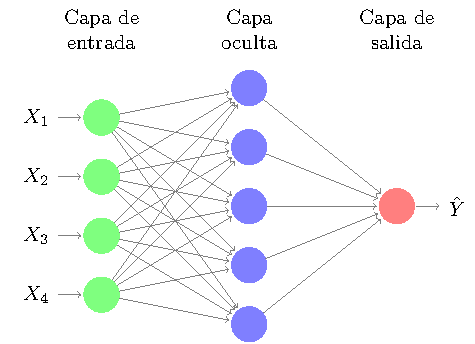
\includegraphics[width=0.8\linewidth]{figuras/neuralNetwork.pdf}
	\caption*{Fuente: elaboración propia, con base en\\ \url{http://www.texample.net/tikz/examples/neural-network/}}
\end{figure}

La capa de entrada recibe las variables explicativas del modelo, de forma análoga con un modelo lineal. La capa de salida es similar a la variable dependiente. Al final de un proceso de entrenamiento, esta capa provee una salida estimada, que puede ser interpretada como la respuesta del modelo a las entradas que no han sido observadas por la red. La capa oculta es crítica para un modelado exitoso, debido a que permite capturar las componentes no observadas en un modelo lineal, y se encarga de capturar la correlación entre las entradas y la salida, lo que provee a la red neuronal con una cierta intuición de predicción e inteligencia en el aprendizaje de los patrones de entrada y salida, ayudando a una correcta inferencia en las relaciones de entradas y salidas no vistas, proceso al que se le conoce como generalización. \parencite{sunythesis} 

%\clearpage

\subsubsection{Principios básicos del modelo de redes neuronales}

Se describe el concepto de función de activación, así como la expresión matemática que representa un modelo de RNA.

\paragraph{Función de activación no lineal}
Una función de activación permite limitar la amplitud de la salida de una neurona. En la figura \ref{ann_structure}, cada una de las neuronas en la capa oculta cuenta con una función de activación.\\

La función de activación se caracteriza cuenta con un grado de no linealidad que permite a la red neuronal detectar y posteriormente reproducir patrones no lineales cuando los datos son muy complejos \parencite{sunythesis}. Debido al algoritmo de entrenamiento utilizado en el ajuste de los pesos sinápticos para una RNAs, la diferenciabilidad es la única condición que debe satisfacer una función de activación \parencite{haykin1999neural}.\\

Los ejemplos de funciones continuamente diferenciables más comúnmente utilizadas en RNAs son las funciones sigmoide logística y tangente hiperbólica. La función logística: \[ \phi(x) = \frac{1}{1 + e^{-x}} \] se utiliza comúnmente en los modelos probabilísticos, mientras que la sigmoide tangente hiperbólica: \[ \phi(x) = \frac{e^x - e^{-x}}{e^x + e^{-x}} \] se utiliza habitualmente en los modelos de regresión, sin embargo, esta última es en realidad la función logística reescalada y sumada a una constante.


\paragraph{Expresión para el modelo de redes neuronales}
% Acá mencionar que la capa de salida tiene una función lineal, debido a que la variable de salida no está acotada en un intervalo
Aunque existen varios tipos de RNAs, las de 3 capas de tipo \textit{feedforward} son las más populares y ampliamente utilizadas, como la que se muestra en la figura \ref{ann_structure}. En la ecuación \ref{ann_model} se muestra la representación más general para una RNA \textit{feedforward} de tres capas, con $J$ neuronas en la capa oculta.

\begin{equation}
	Y = f \bigg ( w_0 + \sum_{j=1}^{J} \phi \big ( w_{0j} + \mathbf{w_j}^T \mathbf{x} \big )\bigg )
	\label{ann_model}
\end{equation}

donde $w_0$ denota un término de intercepto en la neurona de salida, $w_{0j}$ el intercepto en la $j$ neurona oculta, $w_j$ denota el peso sináptico de la $j$ neurona oculta hacia la neurona de salida, $\mathbf{w_j} = (w_{1j}, \ldots, w_{nj})$ el vector de todos los pesos sinápticos de la entrada hacia la neurona $j$, y $\mathbf{x} = (x_1, \ldots, x_n)$ el vector de variables de entrada.\\

Finalmente, $\phi$ representa la función de activación de la capa oculta, y $f$ la función de activación de la neurona de salida. Se hace la distinción debido a que $f$ puede ser la función identidad ($f(x) = x$), que se utiliza generalmente en tratamiento de RNAs como modelos de regresión.

% Técnicas para el modelo de redes neuronales
\subsubsection{Pasos para el desarrollo de la red neuronal}
Para llevar a cabo el desarrollo de la red neuronal, de acuerdo con \textcite{sunythesis}, se deben seguir el siguiente conjunto de pasos:

\begin{enumerate}
	\item Escoger el conjunto de variables explicatorias.

	\item Escoger una arquitectura de RNA adecuada.
	
	\item Seleccionar el número de capas ocultas y el número de neuronas en cada capa oculta, e inicializar los pesos de interconexión.
	
	\item Organizar la muestra en orden temporal ascendente, y dividr los datos en tres conjuntos: de entrenamiento (o ajuste de los pesos), de validación, y de prueba.
	
	\item Utilizar un software para obtener el modelo.
	
	\item Evaluar el desempeño de pronóstico del modelo y comparar con otros modelos lineales y no lineales.
	
	\item Repetir los pasos 3-6 hasta que se alcance el mínimo error de pronóstico sobre el conjunto de validación (el mínimo de la medida de error cuadrático medio).
	
	\item Repetir los pasos 2-7 variando la arquitectura de la red hasta que se alcance un mínimo del error global.
	
	\item Decidir si deben añadirse o removerse variables explicatorias.
	
	\item Finalmente, repetir los pasos 1-9 hasta que se alcance el mínimo error a través de las combinaciones de variables de entrada.
\end{enumerate}


\subsubsection{Elementos técnicos de la red neuronal}
Se describen algunos aspectos relacionados con el entrenamiento y evaluación de la red neuronal.

\paragraph{Normalización de los datos} Para el trabajo se utiliza el logaritmo del tipo de cambio como variable dependiente del modelo, y debido a que se utiliza la función sigmoide tangente hiperbólica, es necesario normalizar los datos de entrada y salida en un rango adecuado, correspondiente al intervalo $(-1, 1)$. Citando a LeCun (1993), cada variable de entrada debe ser preprocesada de tal forma que su valor medio sobre todo el conjunto de entrenamiento esté cercano a cero, o bien, sea pequeño en comparación con su desviación estándar, esto permite acelerar el proceso de aprendizaje de la red neuronal. \parencite{haykin1999neural}.\\

En el trabajo se realiza una normalización de los datos sustrayendo la media de cada una de las variables explicativas y dividiendo por la desviación estándar de la muestra completa (180 observaciones).

\paragraph{Determinación de la arquitectura}
Esta tarea consiste en determinar el número de capas en la red neuronal y el número de elementos en cada capa, lo que determina el número de pesos sinápticos a ser determinados. De acuerdo con \textcite{sunythesis}, seleccionar estos parámetros depende del problema en particular que se desee resolver, debido a que no existe un método teórico sólido que permita seleccionar los mismos.\\

En este trabajo se utiliza una arquitectura de interconexión de cada una de las neuronas con todas las neuronas de la siguiente capa, y se utiliza una arquitectura de una capa oculta, que de acuerdo con el teorema de aproximación universal descrito en \textcite{haykin1999neural}, es suficiente para que una red neuronal artificial compute una aproximación uniforme a un conjunto de entrenamiento representado por el conjunto de entradas\footnote{En \textcite[209]{haykin1999neural} se puede encontrar una descripción completa del teorema.}.\\

En cuanto a la cantidad de neuronas de la capa oculta, se escoge en base a las medidas de error de pronóstico tanto dentro como fuera de la muestra, y finalmente se escogen dos arquitecturas finales para realizar el pronóstico, con ocho y nueve neuronas en su capa oculta.

%Citando a \textcite{haykin1999neural}, el problema con redes neuronales de una sola capa oculta es que las neuronas tienden a interactuar entre sí de forma global, y en situaciones complejas, esta interacción hace difícil mejorar la aproximación en un punto sin empeorarla en otro, mientras que con dos capas ocultas, el proceso de aproximación de curvas se vuelve más manejable.


\paragraph{Algoritmo de entrenamiento}

El algoritmo utilizado para entrenar a la red neuronal se conoce como \textit{backpropagation}, que provee un método computacionalmente eficiente para el ajuste de los pesos sinápticos. La razón por la que este algoritmo adopta este nombre es porque la red es entrenada utilizando los valores de salida deseados, así es posible obtener una medida de error desde la salida, y dicho error es propagado hacia atrás para la modificación (o aprendizaje) de los pesos sinápticos.\\

En este trabajo se utiliza una variante del algoritmo conocida como \textit{resilient backpropagation} (en concreto RPROP+), que modifica los pesos de la red neuronal para encontrar un mínimo local de la función de error. Para esto, el algoritmo computa un gradiente de la función de error respecto a los pesos sinápticos ($dE_{rr}/d\mathbf{w}$) para encontrar una raíz, y en particular, los pesos se modifican en dirección opuesta a las derivadas parciales hasta alcanzar un mínimo local con una cierta medida de tolerancia.

\paragraph{Mínimo global}
En general, no se puede demostrar que el algoritmo de propagación hacia atrás converja, y no hay criterios bien definidos para detener su operación. En su lugar, existen criterios razonables con mérito práctico para terminar el ajuste de pesos. Para formular dichos criterios es necesario pensar en términos de las propiedades de un mínimo local, o global, de la superficie de error \parencite{haykin1999neural}. En este trabajo se utiliza un umbral para las derivadas parciales de la función de error como criterio de parada para el entrenamiento de la red neuronal.\\

En la aplicación de modelos no lineales (como la red neuronal empleada) se tiene la dificultad de que difícilmente se puede saber si se obtuvo un mínimo global en la estimación, porque puede estar enmascarado por muchos mínimos locales con relaciones matemáticas cercanas. Para evitar la introducción de este problema es necesario repetir la estimación utilizando distintos pesos sinápticos iniciales y aleatorios, y finalmente guardar la mejor estimación.



\paragraph{Tamaño de la muestra}
Las RNAs con más observaciones pueden detectar estructuras más complejas y manejar las irregularidades en los datos más efectivamente para alcanzar mayor precisión en el modelado. En este trabajo se utiliza una muestra relativamente larga de 180 observaciones (mensuales de enero de 2001 a diciembre de 2015) para aplicar en la estimación y validación de la red neuronal.



% Finalmente la especifiación del modelo
\subsubsection{Especificación del modelo}

Se utiliza un modelo macroeconómico no lineal $\Phi$ de la forma: 

\[	s_t = \Phi (M_t) + \epsilon_t \]

donde $s_t$ es el logaritmo natural del tipo de cambio $spot$ sobre los meses de observación, y $M_t$ es un vector de variables macroeconómicas, es decir, la oferta relativa de dinero, el ingreso relativo, el diferencial de la tasa de interés, y el diferencial de inflación esperada de largo plazo; $\epsilon_t$ es un término de error aleatorio.\\

La especificación exacta del modelo utilizado es la siguiente:

\begin{equation}
s_t = f(X_{1t}, X_{2t}, X_{3t}, X_{4t}) + \epsilon_t
\label{annModel}
\end{equation}

donde $f$ representa la aproximación de la red neuronal a los datos.\\

% Nuevamente, el pronóstico fuera de la muestra se realiza utilizando las observaciones de las variables explicativas del modelo.

En la figura \ref{fig:ann_monetary9} se muestra el diagrama final de la arquitectura de la red neuronal artificial utilizada para el pronóstico del tipo de cambio, en donde \textit{s} representa el logaritmo natural del tipo de cambio, \textit{m} representa la oferta relativa de dinero, \textit{i} el diferencial de tasas de interés, \textit{y} el diferencial de ingreso real e \textit{inf} el diferencial de inflación esperada.

\begin{figure}[ht]
	\centering
	\caption{Estructura de la red neuronal artificial utilizada para pronóstico}
	\label{fig:ann_monetary9}
	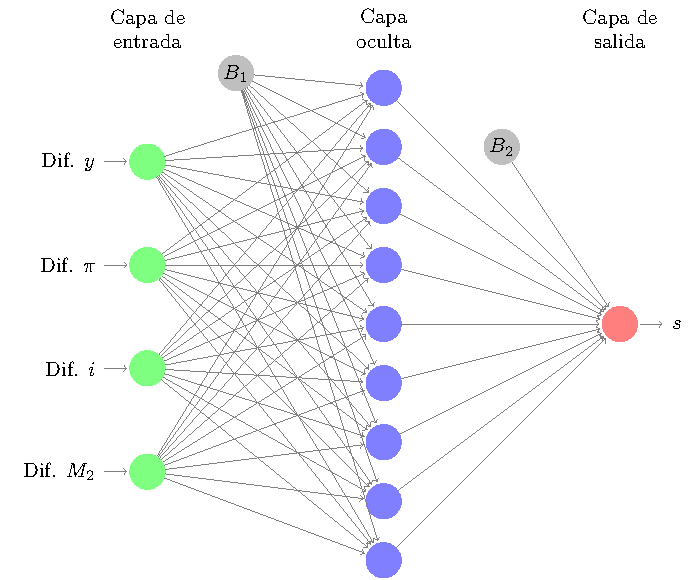
\includegraphics[width=0.8\linewidth]{figuras/spec_ann.pdf}
	\caption*{Fuente: elaboración propia.}
\end{figure}


\subsection{Método de Garson para interpretación de los pesos sinápticos}
Debido a que no existe una interpretación clara de los pesos sinápticos de la red neuronal se utiliza el método de Garson, que identifica la importancia relativa de las variables explicativas para una variable de respuesta de la red neuronal deconstruyendo los pesos del modelo.\\

La idea básica es que la importancia relativa (o fuerza de de asociación) de una variable explicativa para una respuesta específica puede ser determinada identificando todos las conexiones ponderdadas entre los nodos de interés, esto es, se identifican todos los pesos sinápticos que pasan de una entrada específica hacia la capa oculta y finalmente hacia la salida. Finalmente, se obtiene un único valor para cada variable explicativa, que describe la relación con la variable de respuesta de la red neuronal.

% Como se evaluará el modelo: a través de las medidas de pronóstico fuera de la muestra

\subsection{Evaluación del modelo}
Para evaluar el desempeño de los modelos de pronóstico se utilizarán algunas pruebas de especificación dentro de la muestra. El propósito de este trabajo es evaluar el desempeño fuera de la muestra de la red neuronal y compararla con otros modelos. Para cumplir este propósito se guardan las últimas 36 observaciones de la muestra para realizar el pronóstico con los distintos modelos y finalmente contrastar los resultados de acuerdo con las medidas obtenidas.\\

% Una cualidad excepcional de las RNAs es la flexibilidad en la construcción de modelos econométricos, sin embargo, un exceso de flexibilidad puede provocar un problema de sobreajuste (\textit{overfitting}, como se conoce en la literatura) en la red neuronal. Cuando una red neuronal presenta este problema, esta no puede inferir el proceso real de generación de los datos, y afecta negativamente la calidad de los pronósticos.

En este trabajo se utilizan los valores observados de las variables explicativas en los modelos para el pronóstico del tipo de cambio fuera de la muestra, tal como en el trabajo de \textcite{meese1983empirical}, con el objetivo de evaluar la capacidad de inferencia de la RNA sobre los datos.

\subsubsection{Medidas de precisión del pronóstico fuera de la muestra}

La medida de desempeño más importante en una RNA utilizada para pronóstico es la precisión de predicción para observaciones fuera de la muestra. Prácticamente se mide el grado de precisión con el error de pronóstico, que es la diferencia entre el valor observado y el pronosticado.\\

En este trabajo se utiliza como medida de precisión la raíz del error cuadrático medio (RMSE, por sus siglas en inglés), la raíz del error cuadrático medio porcentual (RMSPE), y el Porcentaje de Puntos de Inflexión Correctamente Pronosticados (PERC, por sus siglas en ingleś). El RMSE se puede definir como:

\begin{equation}
	\mathrm{RMSE} = \sqrt{\frac{1}{T} \sum_{t=1}^{T} (Y_t^s - Y_t^a)^2}
	\label{rmsedef}
\end{equation}

donde $Y_t^s$ es el valor estimado (o pronosticado), $Y_t^a$ es el valor observado, y $T$ el número de períodos de pronóstico en los datos. Asimismo, siguiendo la misma notación, el RMSPE se puede definir como: 

\begin{equation}
\mathrm{RMSE} = \sqrt{\frac{1}{T} \sum_{t=1}^{T} (\frac{Y_t^s - Y_t^a}{Y_t^a})^2}
\label{rmspedef}
\end{equation}

El indicador PERC se enfoca en la dirección del pronóstico más que en la precisión de los pronósticos, y sirven para indicar si el modelo puede predecir de forma precisa si el tipo de cambio subirá o bajará en el siguiente período, aunque no necesariamente indique la cantidad. Puede definirse como sigue: 

\begin{equation}
	\mathrm{PERC} = \frac{T_p + T_n}{T}
	\label{percdef}
\end{equation}

donde $T_p$ y $T_n$ representan el número de predicciones correctas con signo positivo y negativo, respectivamente, y $T$ el número total de predicciones.

	
	% Análisis de resultados
	\section{Resultados}

Se presentan los resultados obtenidos en el pronóstico del tipo de cambio utilizando el modelo de caminata aleatoria y los modelos monetarios, en su versión lineal y a través de redes neuronales artificiales de ocho y nueve neuronas.

\subsection{Modelo de caminata aleatoria}
Utilizando la serie de tipo de cambio, se utilizan 144 observaciones mensuales (desde enero de 2001 hasta diciembre de 2013) para pronosticar el tipo de cambio 36 períodos adelante (desde enero de 2013 hasta diciembre de 2015).

\subsubsection{Pronóstico fuera de la muestra}

\begin{figure}[htb]
	\centering
	\caption{Pronóstico del tipo de cambio Q/USD con modelo de caminata aleatoria}
	\label{fig:rwout}
	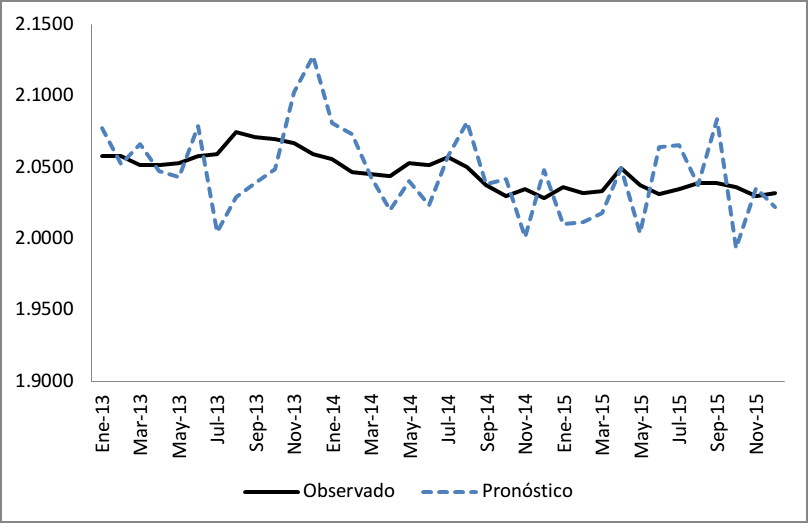
\includegraphics[width=0.9\textwidth]{figuras/RW_out.png}
	\caption*{Fuente: elaboración propia.}
\end{figure}

\clearpage
%\vspace*{1cm}
En la figura \ref{fig:rwout} se muestra el pronóstico del tipo de cambio. Como se puede observar, los valores pronosticados del tipo de cambio siguen la tendencia del tipo de cambio observado.\\

Las medidas de error obtenidas son relativamente pequeñas (RMSE = 0.0276 y RMSPE = 0.0135). Además, el modelo captura correctamente un PERC = 42\% de los puntos de inflexión respecto al aumento o disminución del tipo de cambio en el siguiente período.\\

Finalmente, se puede decir que el modelo presenta mucha volatilidad alrededor de la tendencia del tipo de cambio observado. Esto es debido a que la varianza utilizada para generar la componente aleatoria $\epsilon_t$ del modelo se ve afectada significativamente a inicios de los años 2000 y durante los años 2008 a 2011.

\newpage
\subsection{Modelo monetario lineal}
Utilizando los resultados de un modelo de regresión lineal obtenidos con EViews 9 se obtienen los valores ajustados del tipo de cambio dentro de la muestra de estimación, y los pronósticos del tipo de cambio.\\

En la tabla \ref{tab:estimlin} se muestra la estimación para el modelo monetario lineal. Como se observa, tanto la oferta de dinero, como la inflación no resultan estadísticamente significativas. Asimismo, los signos de la oferta monetaria, el ingreso real, y la tasa de interés no son los esperados de acuerdo con el modelo teórico. Y de acuerdo con el modelo teórico de precios rígidos, la velocidad de ajuste de las desviaciones del tipo de cambio resulta negativa.

\input{tablas/regLineal}

En la estimación del modelo se obtuvo el problema de autocorrelación de los errores, pero debido a que el enfoque de este trabajo consiste en evaluar el desempeño de los modelos de pronóstico, no se realiza ninguna modificación en la estimación del modelo.

\subsubsection{Pronóstico dentro de la muestra}
Utilizando los resultados obtenidos del modelo monetario lineal, se utilizan para obtener los valores ajustados dentro de la muestra. En la figura \ref{fig:linin} se muestra el pronóstico dentro de la muestra para el tipo de cambio.\\

\begin{figure}[htb]
	\centering
	\caption{Ajuste del tipo de cambio Q/USD con modelo monetario lineal}
	\label{fig:linin}
	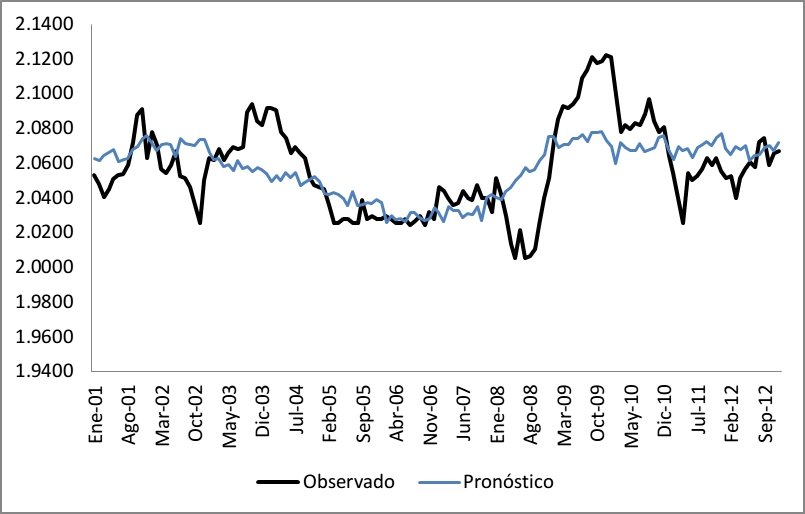
\includegraphics[width=0.7\textwidth]{figuras/lin_in.png}
	\caption*{Fuente: elaboración propia.}
\end{figure}

Como se observa, el modelo monetario lineal se ajusta suavemente a la tendencia del tipo de cambio observado durante el período de estimación, y en general, este no puede explicar las fuertes desviaciones de la tendencia. Respecto a las medidas de error, se obtienen valores relativamente pequeños (RMSE = 0.0208 y RMSPE = 0.0101), y además se obtiene porcentaje de predicción de puntos de inflexión PERC = 55\% de las observaciones dentro de la muestra.

\newpage
\subsubsection{Pronóstico fuera de la muestra}
Con la estimación del modelo se procede a obtener el pronóstico del tipo de cambio, el cual se muestra en la figura \ref{fig:linout}. Como se puede observar, dicho pronóstico sigue una tendencia relativamente constante y no logra percibir la caída del tipo de cambio a partir de septiembre de 2013.\\

\begin{figure}[htb]
	\centering
	\caption{Pronóstico del tipo de cambio Q/USD con modelo monetario lineal}
	\label{fig:linout}
	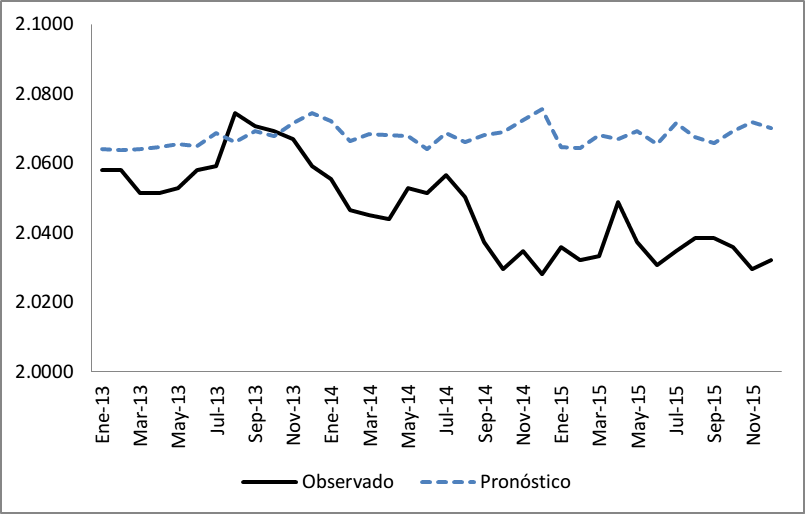
\includegraphics[width=0.7\textwidth]{figuras/lin_out.png}
	\caption*{Fuente: elaboración propia.}
\end{figure}

En cuanto a las medidas de error, presenta menores valores que el modelo de caminata aleatoria (RMSE = 0.0251 y RMSPE = 0.0123) y una mayor tasa de predicción de puntos de inflexión (PERC = 43\% de 36 observaciones fuera de la muestra).

\clearpage

\subsection{Modelo monetario de RNA con 8 neuronas}
Se ajusta una RNA de una capa oculta con ocho neuronas utilizando las variables normalizadas como se menciona en la metodología. 
% Esto va en la metodología
Asimismo, la elección de la arquitectura de la red neuronal se decide por las medidas de error de pronóstico, tanto adentro como afuera de la muestra.

\subsubsection{Pronóstico dentro de la muestra}
En la figura \ref{fig:annin18} se muestran los valores pronosticados dentro de la muestra para el tipo de cambio. Se puede observar que la red neuronal aprende sobresalientemente ($R^2 = 0.91$) el patrón de comportamiento del tipo de cambio dentro de la muestra de entrenamiento. Asimismo, exhibe medidas de error más bajas que las del modelo de caminata aleatoria y del modelo lineal (RMSE = 0.0076 y RMSPE = 0.0037). Y finalmente, logra predecir correctamente un 72\% (sobre las 144 observaciones) de los puntos de inflexión de la muestra.

\begin{figure}[htb]
	\centering
	\caption{Ajuste del tipo de cambio Q/USD con modelo de RNAs 8 neuronas}
	\label{fig:annin18}
	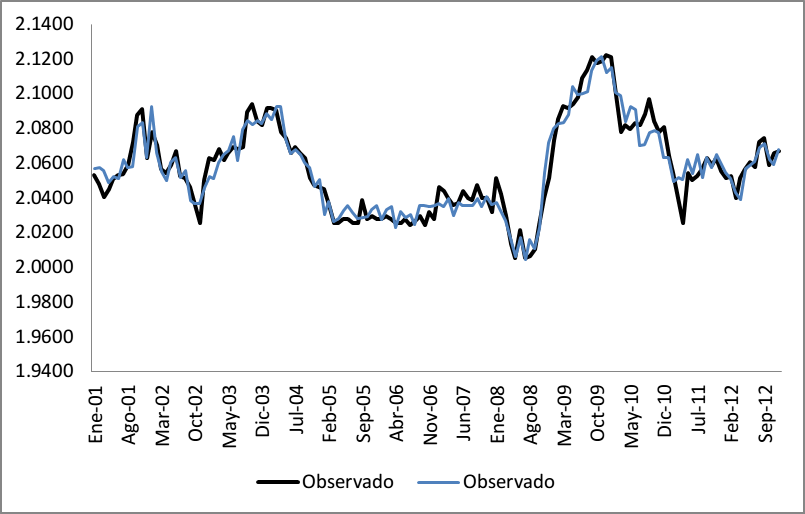
\includegraphics[width=0.7\textwidth]{figuras/ann18_in.png}
	\caption*{Fuente: elaboración propia.}
\end{figure}

\subsubsection{Pronóstico fuera de la muestra}

En la figura \ref{fig:annout18} se muestra el pronóstico de la red neuronal utilizando valores fuera de la muestra de entrenamiento. Como se puede observar, la red neuronal predice con mejor precisión la volatilidad en el tipo de cambio porque aprende el patrón de movimiento de las variables, lo que lleva a una mejor predicción del tipo de cambio. Y aunque existe un sesgo de nivel en la predicción del modelo sobre el tipo de cambio observado, la red neuronal consigue un balance entre la explicación de la volatilidad y el nivel del tipo de cambio. 

\begin{figure}[htb]
	\centering
	\caption{Pronóstico del tipo de cambio Q/USD con modelo de RNAs 8 neuronas}
	\label{fig:annout18}
	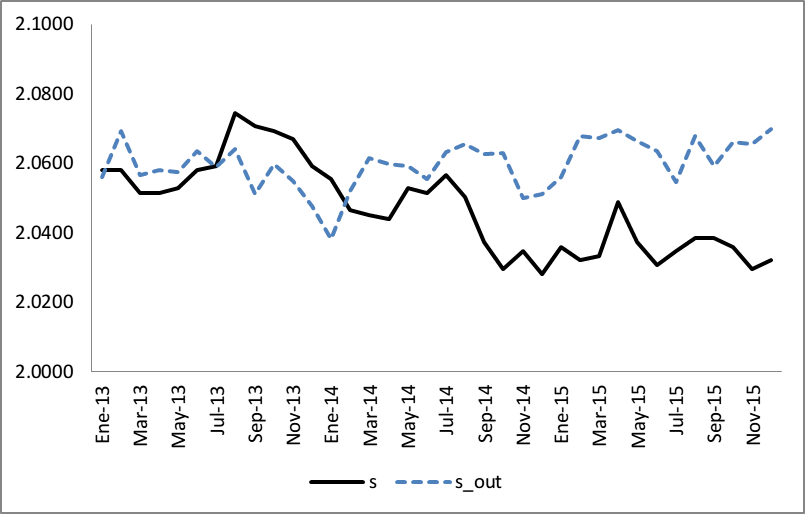
\includegraphics[width=0.7\textwidth]{figuras/ann18_out.png}
	\caption*{Fuente: elaboración propia.}
\end{figure}

En cuanto a las medidas de error, el pronóstico fuera de la muestra exhibe menores indicadores que el modelo lineal y el modelo de caminata aleatoria (RMSE = 0.02059 y RMSPE = 0.01011). Y en cuanto al pronóstico de puntos de inflexión, logra predecir un 57\% sobre las 36 observaciones fuera de la muestra, porcentaje que es mayor al indicador obtenido por el modelo lineal y el de caminata aleatoria.



\subsection{Modelo monetario de RNA con 9 neuronas}
Se repite el experimento de entrenamiento de una RNA con una capa oculta y nueve neuronas.

\subsubsection{Pronóstico dentro de la muestra}
En la figura \ref{fig:annin19} se muestran los valores pronosticados dentro de la muestra para el tipo de cambio. Nuevamente, la red neuronal se ajusta extraordinariamente ($R^2 = 0.92$) al patrón de comportamiento del tipo de cambio dentro de la muestra de entrenamiento. Asimismo, exhibe medidas de error más bajas que las del modelo de caminata aleatoria y del modelo lineal (RMSE = 0.0070 y RMSPE = 0.0034). Y finalmente, logra predecir correctamente un 73\% (sobre las 144 observaciones) de los puntos de inflexión de la muestra. En comparación con la red neuronal de ocho neuronas, este modelo se desempeña ligeramente mejor en las medidas de error de pronóstico, y relativamente peor en la predicción correcta de puntos de inflexión.

\begin{figure}[htb]
	\centering
	\caption{Ajuste del tipo de cambio Q/USD con modelo de RNAs 9 neuronas}
	\label{fig:annin19}
	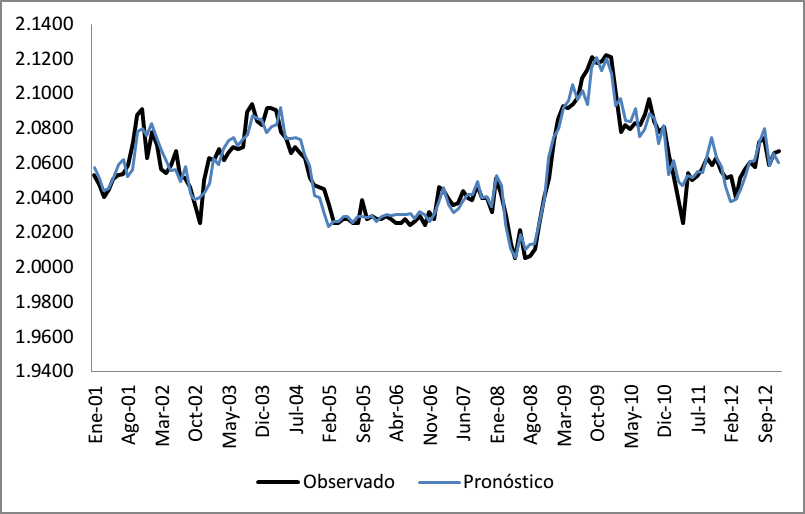
\includegraphics[width=0.7\textwidth]{figuras/ann19_in.png}
	\caption*{Fuente: elaboración propia.}
\end{figure}


\subsubsection{Pronóstico fuera de la muestra}

En la figura \ref{fig:annout19} se muestra el pronóstico de la red neuronal utilizando valores fuera de la muestra de entrenamiento. Como se puede observar, la red neuronal predice con mejor precisión la volatilidad en el tipo de cambio porque aprende el patrón de movimiento de las variables, lo que lleva a una mejor predicción del tipo de cambio. Y aunque existe un sesgo de nivel en la predicción del modelo sobre el tipo de cambio observado, la red neuronal consigue un balance entre la explicación de la volatilidad y el nivel del tipo de cambio. 

\begin{figure}[htb]
	\centering
	\caption{Pronóstico del tipo de cambio Q/USD con modelo de RNAs 9 neuronas}
	\label{fig:annout19}
	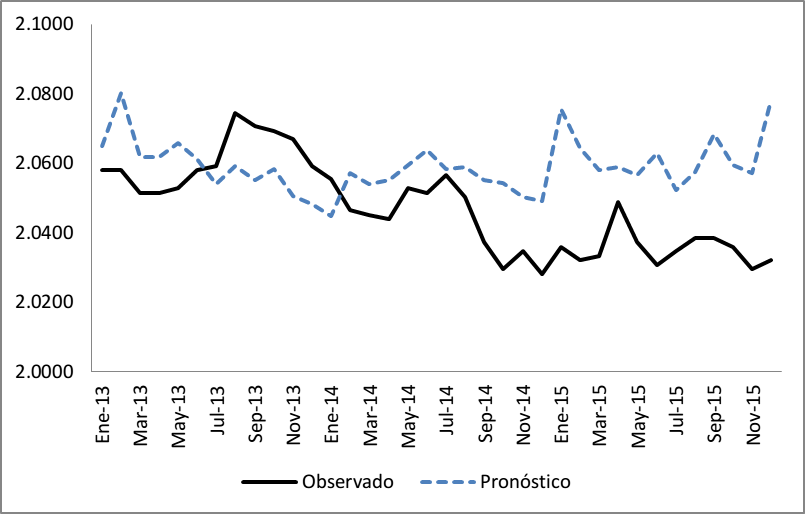
\includegraphics[width=0.7\textwidth]{figuras/ann19_out.png}
	\caption*{Fuente: elaboración propia.}
\end{figure}

En cuanto a las medidas de error, el pronóstico fuera de la muestra exhibe menores indicadores que el modelo lineal y el modelo de caminata aleatoria (RMSE = 0.01969 y RMSPE = 0.00966). Y en cuanto al pronóstico de puntos de inflexión, logra predecir un 46\% sobre las 36 observaciones fuera de la muestra, porcentaje que es mayor al indicador obtenido por el modelo lineal y el de caminata aleatoria.


\subsection{Importancia relativa de variables}
En la figura \ref{fig:importrel18} se muestra el gráfico de importancia relativa para cada una de las variables explicativas del modelo con nueve neuronas, donde \textit{m} representa la oferta relativa de dinero, \textit{i} el diferencial de tasas de interés, \textit{y} el diferencial de ingreso real e \textit{inf} el diferencial de inflación esperada.

\begin{figure}[htb]
	\centering
	\caption{Importancia relativa en el modelo de RNAs con 8 neuronas}
	\label{fig:importrel18}
	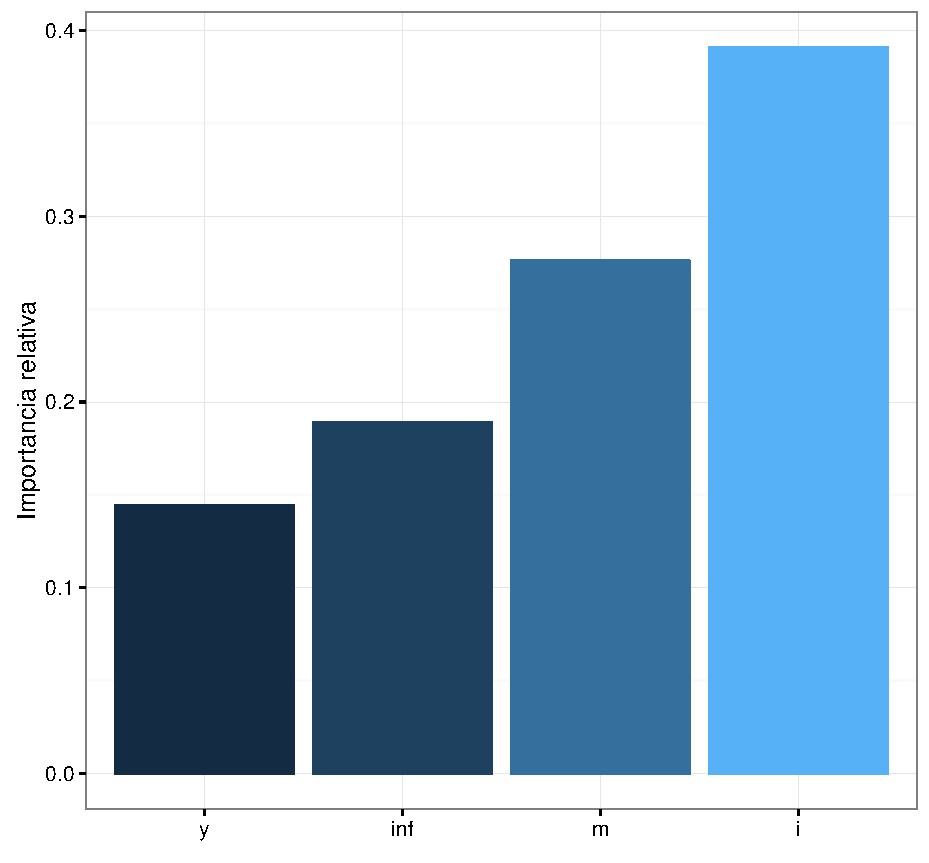
\includegraphics[width=0.6\textwidth]{figuras/garson_18.pdf}
	\caption*{Fuente: elaboración propia.}
\end{figure}

De acuerdo con la importancia relativa de Garson, el ingreso real y la inflación contribuyen muy poco en la explicación del tipo de cambio, mientras que la oferta relativa de dinero y el diferencial de tasas de interés tienen un impacto más significativo sobre el tipo de cambio.\\

\newpage
En la figura \ref{fig:importrel19} se muestra el gráfico de importancia relativa para la red neuronal con nueve neuronas en la capa oculta. Como se puede observar, se reafirma la contribución significativa del diferencial de tasas de interés y de la oferta relativa de dinero.

\begin{figure}[htb]
	\centering
	\caption{Importancia relativa en el modelo de RNAs con 9 neuronas}
	\label{fig:importrel19}
	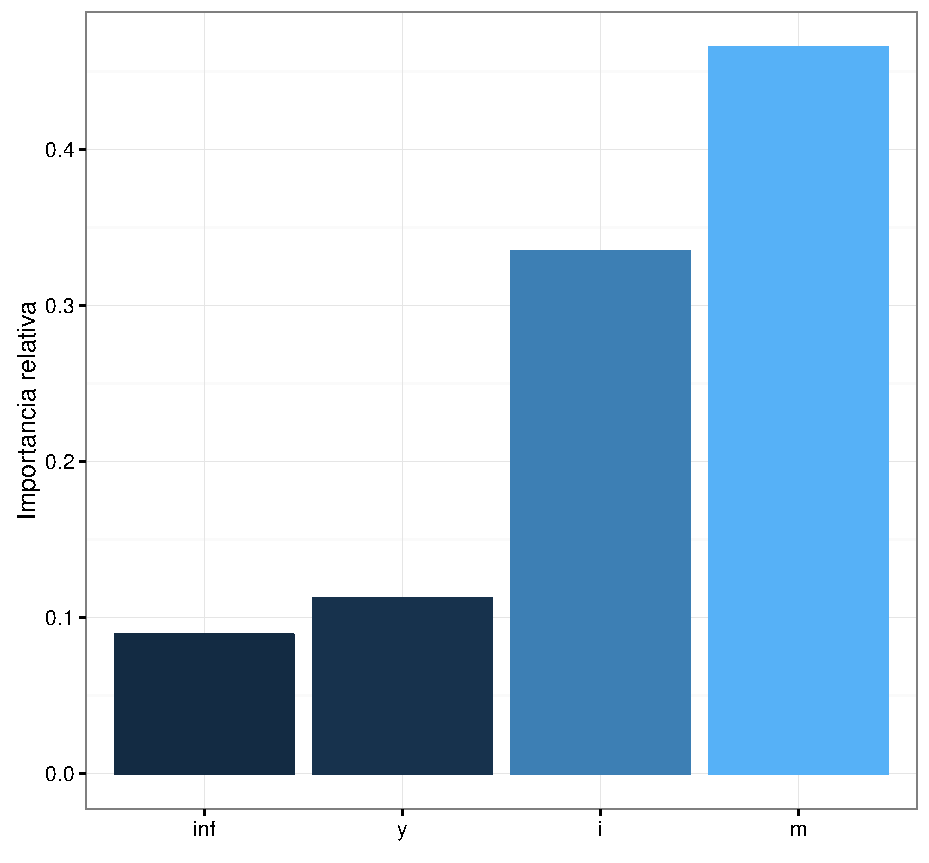
\includegraphics[width=0.6\textwidth]{figuras/garson_19.pdf}
	\caption*{Fuente: elaboración propia.}
\end{figure}

\clearpage
\subsection{Análisis de resultados}
De acuerdo con las medidas de error de pronóstico obtenidas para cada uno de los modelos, como se resumen en la tabla \ref{tab:resOutOfSample}, ambos modelos de redes neuronales proveen un mejor pronóstico en magnitud que los modelos de caminata aleatoria y el modelo lineal, en concordancia con los criterios de RMSE y RMSPE.\\

% Table generated by Excel2LaTeX from sheet 'Tablas'
\begin{table}[htbp]
  \centering
  \caption{Resultados de pronóstico del tipo de cambio Q/USD}
    \begin{tabular}{lrrr}
    \toprule
    \multicolumn{1}{c}{\textbf{Fuera de la muestra}} & \multicolumn{1}{c}{\textbf{RMSE}} & \multicolumn{1}{c}{\textbf{RMSPE}} & \multicolumn{1}{c}{\textbf{PERC}} \\
    \midrule
    Caminata aleatoria    & 0.02763 & 0.01347 & 31\% \\
    Modelo lineal & 0.02512 & 0.01234 & 43\% \\
    RNA con 8 neuronas & 0.02059 & 0.01011 & 57\% \\
    RNA con 9 neuronas & 0.01969 & 0.00966 & 46\% \\
    \bottomrule
    \end{tabular}%
    \caption*{Fuente: elaboración propia.}
  \label{tab:resOutOfSample}%
\end{table}%


En cuanto a la predicción de puntos de inflexión, el modelo monetario lineal supera al de caminata aleatoria, y asimismo, los modelos de RNAs exhiben porcentajes más altos que los del modelo lineal, siendo superior el modelo que utiliza ocho neuronas en la capa oculta.\\

En la tabla \ref{tab:ratioError} se muestra el resumen del cociente de error entre los modelos monetarios y el modelo de caminata aleatoria. Como se puede observar, tanto el modelo monetario lineal como el modelo de redes neuronales poseen una relación de error menor a 1, lo que indica que el modelo de caminata aleatoria posee el peor desempeño de pronóstico del tipo de cambio del quetzal. Es decir, este resultado apoya la hipótesis de que la predicción del tipo de cambio sí se puede llevar a cabo con los fundamentos macroeconómicos, y que toda la información disponible en la serie del tipo de cambio no es suficiente para pronosticar el comportamiento del mismo.\\

% Table generated by Excel2LaTeX from sheet 'Tablas'

\begin{table}[htbp]
	\centering
	\caption{Relación de error entre modelos de pronóstico}
	\begin{tabular}{lrr}
		\toprule
		\textbf{Modelo} & \textbf{RMSE/RW} & \textbf{RMSPE/RW} \\
		\midrule
		Lineal & 0.9090 & 0.9156 \\
		%RNA\_18 & 0.7452 & 0.7502 \\
		Red neuronal & 0.7127 & 0.7171 \\
		\bottomrule
	\end{tabular}%
	\label{tab:ratioError}%
	\caption*{Fuente: elaboración propia.}
\end{table}


Asimismo, como se observa en la tabla \ref{tab:ratioError}, las medidas de error de pronóstico del tipo de cambio para el modelo no lineal (RNA) son menores que las del modelo lineal, esto indica que existe una relación no lineal inherente entre las variables macroeconómicas que determinan el tipo de cambio, y que utilizando una relación no lineal entre las variables es posible explicar mejor las variaciones del tipo de cambio.\\

En cuanto a la interpretación de las variables que determinan el tipo de cambio, de acuerdo con el modelo monetario lineal, el diferencial de tasas de interés entre Guatemala y Estados Unidos es un determinante clave, y aunque resulte con un signo contrario al esperado, este resultado se confirma a través de las gráficas de importancia relativa extraídas de los modelos de redes neuronales, que asignan un grado de importancia sobresaliente al diferencial de tasas de interés y a la oferta de dinero, que resulta no significativa en el modelo lineal. Este resultado puede reflejar la tendencia de Guatemala a seguir en cierta medida las acciones de política monetaria de países desarrollados como Estados Unidos, ya que precisamente son las variables monetarias las que determinan el tipo de cambio en Guatemala.\\

Finalmente, el modelo monetario con redes neuronales provee el mejor resultado de pronóstico en magnitud y dirección para el caso de Guatemala y Estados Unidos. Y en este caso fue posible superar la prueba planteada por \textcite{meese1983empirical} de superar el pronóstico del tipo de cambio dado por una caminata aleatoria con un modelo estructural no lineal que utiliza fundamentos macroeconómicos.


	
	% Observaciones finales
	\section{Observaciones finales}

Las principales observaciones de este trabajo son: 

\begin{itemize}
	%\item Las redes neuronales artificiales conforman un método no lineal de estimación de modelos econométricos que permite realizar pronósticos, ya que pueden aprender el patrón de movimiento de las variables, y en cierta medida sirven para comprobar la relación existente entre las variables explicativas y la variable respuesta del modelo.
	
	\item Las redes neuronales artificiales conforman un método no lineal de estimación de modelos econométricos que permitieron realizar pronósticos, ya que pueden aprender el patrón de movimiento de las variables, y en cierta medida sirven para comprobar la relación existente entre el tipo de cambio y otras variables explicativas del modelo monetario. Finalmente, el modelo de redes neuronales artificiales en la predicción del tipo de cambio mostró los mejores resultados tanto en magnitud como dirección de los pronósticos, en comparación con un modelo monetario lineal, y con uno de caminata aleatoria.
	
	\item Se pudo pronosticar el tipo de cambio en Guatemala en un corto y mediano plazo a partir de los fundamentos macroeconómicos de un modelo monetario, resultado que va en contra del paradigma actual de la literatura, en el cual no es posible obtener mejores pronósticos que con un modelo de caminata aleatoria.
	
	\item En cuanto a la importancia de las variables explicativas, el modelo monetario lineal y el de redes neuronales resaltan la importancia del diferencial de tasas de interés entre Guatemala y Estados Unidos, así como la importancia de la oferta monetaria relativa mostrada por el modelo de redes neuronales, lo que indica que el tipo de cambio está principalmente explicado por las variables  guiadas a través de la política monetaria de Guatemala y Estados Unidos.
\end{itemize}
	
	% Bibliografía
	%\nocite{*}
	\printbibliography[heading=bibintoc]
	
	% Anexos
	\section*{Anexos}
\addcontentsline{toc}{section}{Anexos}

\subsection*{Prueba de Diebold-Mariano: precisión predictiva entre pronósticos}

\textcite{diebold1995comparing} desarrollaron una prueba para comparar la precisión de pronóstico entre dos modelos. Utilizando una función de pérdida $g(\cdot)$ sobre el error de pronóstico fuera de la muestra $e_{it} = \hat{y}_{it} - y_{t}$, donde $i$ representa el número de modelo ($i = 1,2$), $\hat{y}_{it}$ representa el pronóstico del modelo $i$ en la observación $t$ fuera de la muestra, y $y_{t}$ el valor observado. Finalmente, se define la pérdida diferencial entre los modelos como \[ d_t = g(e_{1t}) - g(e_{2t}) \] 

La idea principal de la prueba consiste en probar que los dos modelos tienen la misma pérdida de predicción, por lo tanto se quiere probar la hipótesis nula de que las pérdidas de predicción son las mismas. En otras palabras, se quiere probar que $ H_0 = E(d_t) = 0 \quad \forall t $. Finalmente, en el trabajo se utiliza un programa de \textit{R} para computar los resultados de la prueba de Diebold y Mariano sobre los modelos de pronóstico presentados anteriormente.\\

En la tabla \ref{tab:dmtest} se comparan los modelos de pronóstico utilizados en el trabajo, y se realiza una prueba Diebold-Mariano de \textit{Modelo 1} contra \textit{Modelo 2}, en la cual la hipótesis nula es que ambos modelos tienen la misma precisión de pronóstico, y la hipótesis alternativa es que el \textit{Modelo 2} tiene menor precisión de pronóstico. La prueba se realiza con utilizando valores de horizonte de pronóstico de hasta 10 meses, y en las columnas se muestra los modelos que se utilizaron para la prueba, y el valor p de la prueba.\\

Como se puede observar en la segunda y cuarta columna, el modelo de redes neuronales artificiales con 9 neuronas es siempre más preciso en pronóstico que el modelo de caminata aleatoria. Asimismo, de acuerdo a la tercera y quinta columna, entre el modelo de caminata aleatoria y el modelo lineal la prueba es rechazada a cualquier nivel de significancia aceptable, por lo que estos tienen diferentes niveles de precisión. Finalmente, observando la sexta columna se puede determinar que el modelo de RNAs con 9 neuronas es posee mayor precisión de pronóstico que el modelo lineal.

% Table generated by Excel2LaTeX from sheet 'Hoja1'
\renewcommand{\baselinestretch}{1.5}
\begin{table}[htb]
  \centering
  \caption{Comparación entre modelos de pronóstico con horizonte de 10 meses}
    \begin{tabular}{cccccc}
    \toprule
    \multicolumn{1}{l}{Modelo 1} & Camin. Aleat. & Camin. Aleat. & RNA9  & Lineal & RNA9 \\
    \multicolumn{1}{l}{Modelo 2} & RNA9  & Lineal & Camin. Aleat. & Camin. Aleat. & Lineal \\
    \midrule
    Horizonte & \multicolumn{5}{c}{Valor p} \\
    \midrule
    \multicolumn{1}{c}{1} & 0.9492 & 0.1491 & 0.0508 & 0.8509 & 0.0272 \\
    \multicolumn{1}{c}{2} & 0.9312 & 0.1832 & 0.0688 & 0.8168 & 0.0260 \\
    \multicolumn{1}{c}{3} & 0.9386 & 0.1883 & 0.0614 & 0.8117 & 0.0304 \\
    \multicolumn{1}{c}{4} & 0.9447 & 0.1969 & 0.0553 & 0.8031 & 0.0471 \\
    \multicolumn{1}{c}{5} & 0.9166 & 0.2284 & 0.0834 & 0.7716 & 0.0506 \\
    \multicolumn{1}{c}{6} & 0.8694 & 0.2689 & 0.1306 & 0.7311 & 0.0518 \\
    \multicolumn{1}{c}{7} & 0.8704 & 0.2744 & 0.1296 & 0.7256 & 0.0525 \\
    \multicolumn{1}{c}{8} & 0.8760 & 0.2785 & 0.1240 & 0.7215 & 0.0778 \\
    \multicolumn{1}{c}{9} & 0.8757 & 0.2863 & 0.1243 & 0.7137 & 0.1112 \\
    \multicolumn{1}{c}{10} & 0.8807 & 0.2870 & 0.1193 & 0.7130 & 0.1058 \\
    \bottomrule
    \end{tabular}%
    \caption*{Fuente: elaboración propia.}
  \label{tab:dmtest}%
\end{table}%
\renewcommand{\baselinestretch}{1.5}


\newpage
\subsection*{Código de \textit{R} para prueba de Diebold y Mariano}

En el código \ref{lst:dmtest} se muestra el programa de \textit{R} utilizado para realizar la prueba de Diebold y Mariano descrita en la sección anterior.

\renewcommand{\baselinestretch}{1}
\lstinputlisting[
	caption={Cómputo de prueba Diebold y Mariano en \textit{R}}, 
	firstline=8, 
	lastline=31,
	label={lst:dmtest}]{listings/dmtest.r}
\renewcommand{\baselinestretch}{1.5}


\newpage
\subsection*{Código de \textit{R} para entrenamiento de red neuronal artificial}
En el código \ref{lst:entann} se muestra el programa de \textit{R} utilizado para el entrenamiento y pronóstico utilizando una red neuronal artificial con el paquete \textit{neuralnet}.

\renewcommand{\baselinestretch}{1}
\lstinputlisting[caption={Programa para entrenamiento de la red neuronal},label={lst:entann}]{listings/ann_pronostico.r}
\renewcommand{\baselinestretch}{1.5}

	
	
\end{document}